%% We use `subfiles' package
\documentclass[preamble.tex]{subfiles}
\begin{document}

\chapter{Equational Fusion Systems}
\label{sec:Equational-Fusion-Systems}
\ieqfusion{}

This section will review two approaches to compile-time fusion in \Haskell: \name{foldr/build} short cut fusion and \name{Stream Fusion}. They both fall into the category of \*equational* fusion systems meaning that they rely on compiler's \*rewrite rules* \cite{PTH01} for them to work.

A major problem with this approach is that it cannot fuse a producer into multiple consumers which is vital for \name{Data Parallel Haskell} as discussed in Section~\ref{sec:problems}.


\clearpage

\section{\name{foldr/build} fusion}
\label{sec:foldr-build}

\name{foldr/build} short cut fusion \cite{GLP93} is one of the most referenced techniques for fusion in \Haskell. It has been developed for use in \GHC to fuse pipelined list operations. It employs two combinators, @foldr@ and @build@, and a single rewrite rule to eliminate adjacent occurrences of the combinators. It is suitable for use in the cases when the functions to be fused can be defined in terms of these combinators. The definition of @foldr@ is reused from \name{Prelude} -- \Haskell's standard library:

\begin{hscode}
foldr :: (a -> b -> b) -> b -> [a] -> b
foldr f z []     = z
foldr f z (x:xs) = f x z : (foldr f z xs)
\end{hscode}


To understand the motivation behind short cut fusion one may think of @foldr@ as of replacing each @Cons@ of a list with a binary operator and @Nil@ with the neutral element. The other combinator, @build@, takes a second order function which in turn takes an operator to be used as @Cons@, and a value to be used as @Nil@. Since we are building a list, these immediately become @(:)@ and @[ ]@.

\begin{hscode}
build :: ((a -> b -> b) -> b -> b) -> [a]
build g = g (:) []
\end{hscode}


To illustrate the approach a @map@ could be defined in terms of @build/foldr@ as follows:

\begin{hscode}[mathescape]
map f xs = build (\c n -> foldr (c . f) n xs)
-- c is $\mathtt{(:)}$, n is $\mathtt{[\ ]}$
\end{hscode}


In the above code the list is being folded into another list. With the help of a rewrite rule

$\langle \mathit{foldr/build\ fusion} \rangle \forall g\, k\, z.\mathit{foldr}\, k\, z\,(build\, g)\mapsto g\, k\, z$

the two consecutive @map@s could be reduced to as in the following:

\begin{hscode}[mathescape]
map h (map f xs)
 -- inline
 = build(\c n -> foldr (c.h) n 
  (build (\c n -> foldr (c.f) n xs)))
 -- apply rewrite rule
 = build(\c n -> ((\c n -> foldr (c.f) n xs) (c.h) n)
 -- $\beta$-reduce
 = build(\c n -> foldr (c.h.f) n xs)
\end{hscode}


While this leads to the desired results in many cases, it requires the programmer to define the functions in a less readable form. This may be acceptable for some of the code in the standard library but is not likely to be widely accepted among client programmers. Thus the fusion breaks for the parts of the code that do not use the explicit @foldr/build@ definitions. To solve this, Chitil proposed a type inference algorithm to automatically infer the @foldr/build@ definitions \cite{Chi99}.

The above limiting factor is critical to the application of the fusion system to lists but is less relevant to \LiveFusion system since the number of combinators is fixed.

However, the limitations that do make it unattractive are the inability to effectively fuse left @fold@s and @zip@s which are both crucial to \DPH. The inability to fuse into multiple consumers is likewise very considerable for such application of the technique as \DPH.


\clearpage

\section{Stream Fusion}
\label{sec:stream-fusion}
\istreamfusion{}

\name{Stream Fusion} \cite{CLS07,CSL06} is originally employed in the \DPH backend library at one of the two levels of fusion discussed in Section~\ref{sec:DPH-fusion-levels}.

It introduces two data types: a \term{stream} and a \term{stepper}.

\begin{hscode}
data Stream a = forall s. Stream (s -> Step s a) s
\end{hscode}


A \*Stream* is defined by its \term{stepper function} and \term{seed}. The \term{seed} is essentially the state of the stream at any given point. The stepper is used to produce a stream by taking the current \*seed* and yielding the \*next step*. That is, the stepper function may produce the next \*element* and \*new state* from \*current state*. The step produced by calling stepper on stream may be one of the following:


\begin{hscode}
data Step s a = Yield a s
              | Skip s
              | Done
\end{hscode}


A @Done@ flags the end of the stream, while @Yield@ contains an element and the new seed (i.e. new state). If a @Skip@ is encountered it means that the current step did not contain an element but the stream has not yet finished\footnote{For example if the stream has skipped an element that did not satisfy the predicate of a \code{filter} combinator.}.

The streaming of a list could be defined in the following way:

\begin{hscode}
stream :: [a] -> Stream a
stream step0 = Stream next step0
  where next []     = Done
        next (x:xs) = Yield x xs
\end{hscode}


The list itself is being used as the seed. Unstreaming back to a list takes the following form:


\begin{hscode}
unstream :: Stream a -> [a]
unstream (Stream next0 step0) = unfold step0
  where unfold s = case next0 s of
          Done       -> []
          Skip s'    -> unfold s'
          Yield x s' -> x : unfold s'
\end{hscode}


Any fusible list function should now be defined in terms of Streams as opposed to lists. For example the @map@ combinator is defined as follows:


\begin{hscode}
mapS :: (a -> b) -> Stream a -> Stream b
mapS f (Stream next0 s0) = Stream next s0
  where next s = case next0 s of
    Done       -> Done
    Skip    s' -> Skip        s'
    Yield x s' -> Yield (f x) s'

map :: (a -> b) -> [a] -> [b]
map f xs = unstream . mapS f . stream
\end{hscode}


Note that the user-facing definition of @map@ still takes a regular lists but converts the list to a stream internally.

To see how a @Skip@ step might be used it may be worthwhile to look at the definition of the @filter@ function.

\begin{hscode}
filterS :: (a -> Bool) -> Stream a -> Stream a
filterS p (Stream next0 s0) = Stream next s0
  where next s = case next0 s of
    Done                   -> Done
    Skip    s'             -> Skip    s'
    Yield x s' | p x       -> Yield x s'
               | otherwise -> Skip    s'

filter :: (a -> Bool) -> [a] -> [a]
filter p = unstream . filterS p . stream
\end{hscode}

Again, the user-facing filter function @stream@s the list before passing it to the stream-based counterpart.

Given the above definitions of @map@ and @filter@ the fusion opportunity such as @map f . filter p@ may now be exploited with the following rewrite rule

$\langle \mathit{stream/unstream\ fusion}\rangle\, \forall stream\, (unstream\, s)\mapsto s$

\begin{hscode}
(map f . filter p) xs
  -- inline definitions of map and filter
  = (unstream . mapS f . stream . unstream . filterS p) xs
  -- apply stream/unstream rewrite rule
  = (unstream . mapS f . filterS p . stream) xs
\end{hscode}

The fusion is not complete at this point but the stream processing functions @mapS@ and @filterS@ are not adjacent and can be fused by inlining the definitions and \GHC's built-in optimisations. In order to completely remove all traces of the helper data structures Stream Fusion relies on general purpose compiler optimisations and a \*Constructor Specialisation* optimisation \cite{SpecConstr}.

A more thorough description list combinator fusion using Stream Fusion can be found in \cite{CLS07}.

\name{Stream Fusion} has proven to be very potent for array processing and is successfully employed in the \name{Vector} library. It can fuse more types of combinators than \name{forldr/build} and \name{Functional Array Fusion} and has recently been extended to support vectorised CPU instructions \cite{VectorStreamFusion}.


%%%%%%%%%%%%%%%%%%%%%%%%%%%%%%%%%%%%%%%%%%%%%%%%%%%%%%%%%%%%%%%%%%%%%%%%%%%%%%%
%%
%% The following section on Functional Array Fusion is excluded.
%%
%%%%%%%%%%%%%%%%%%%%%%%%%%%%%%%%%%%%%%%%%%%%%%%%%%%%%%%%%%%%%%%%%%%%%%%%%%%%%%%

\begin{comment}

\clearpage

\subsection{Functional Array Fusion}

This last approach will be described by first developing an intuition that would lead to the solution more thoroughly described in \cite{CK01,CK03}. We will go to a greater depth describing this approach since it lays down the basis for the work presented.

When talking about fusion it it important to do so with reference to the context. In our case the interface to the primitive library is limited by a number of predefined functions. This is contrary to the approaches that optimising compilers take for fusing generic free-form loops \cite{KA02}. Now that we have established that the interface to the arrays is fixed it is worthwhile to consider the types of operations it offers. Quite expectedly it follows some of the Haskell Prelude conventions as well as the client interface to DPH (Figure \vref{lst:DPH-interface}).

Suppose that one of the evaluation paths of the program arrives at the following computation:

\begin{hscode}
fold (+) 0 (filter isPrime (map (+1) (map (^2) (enumFromTo 0 9))))
\end{hscode}


The dependence graph \cite{RMKB06,KA02} for this computation is presented on the left of Figure \vref{fig:Prime-Sum-evaluation}. One of the ways in which the library functions can be classified is by the types of their arguments and return types. We only focus on whether the function produces or consumes array(s).

\begin{figure}
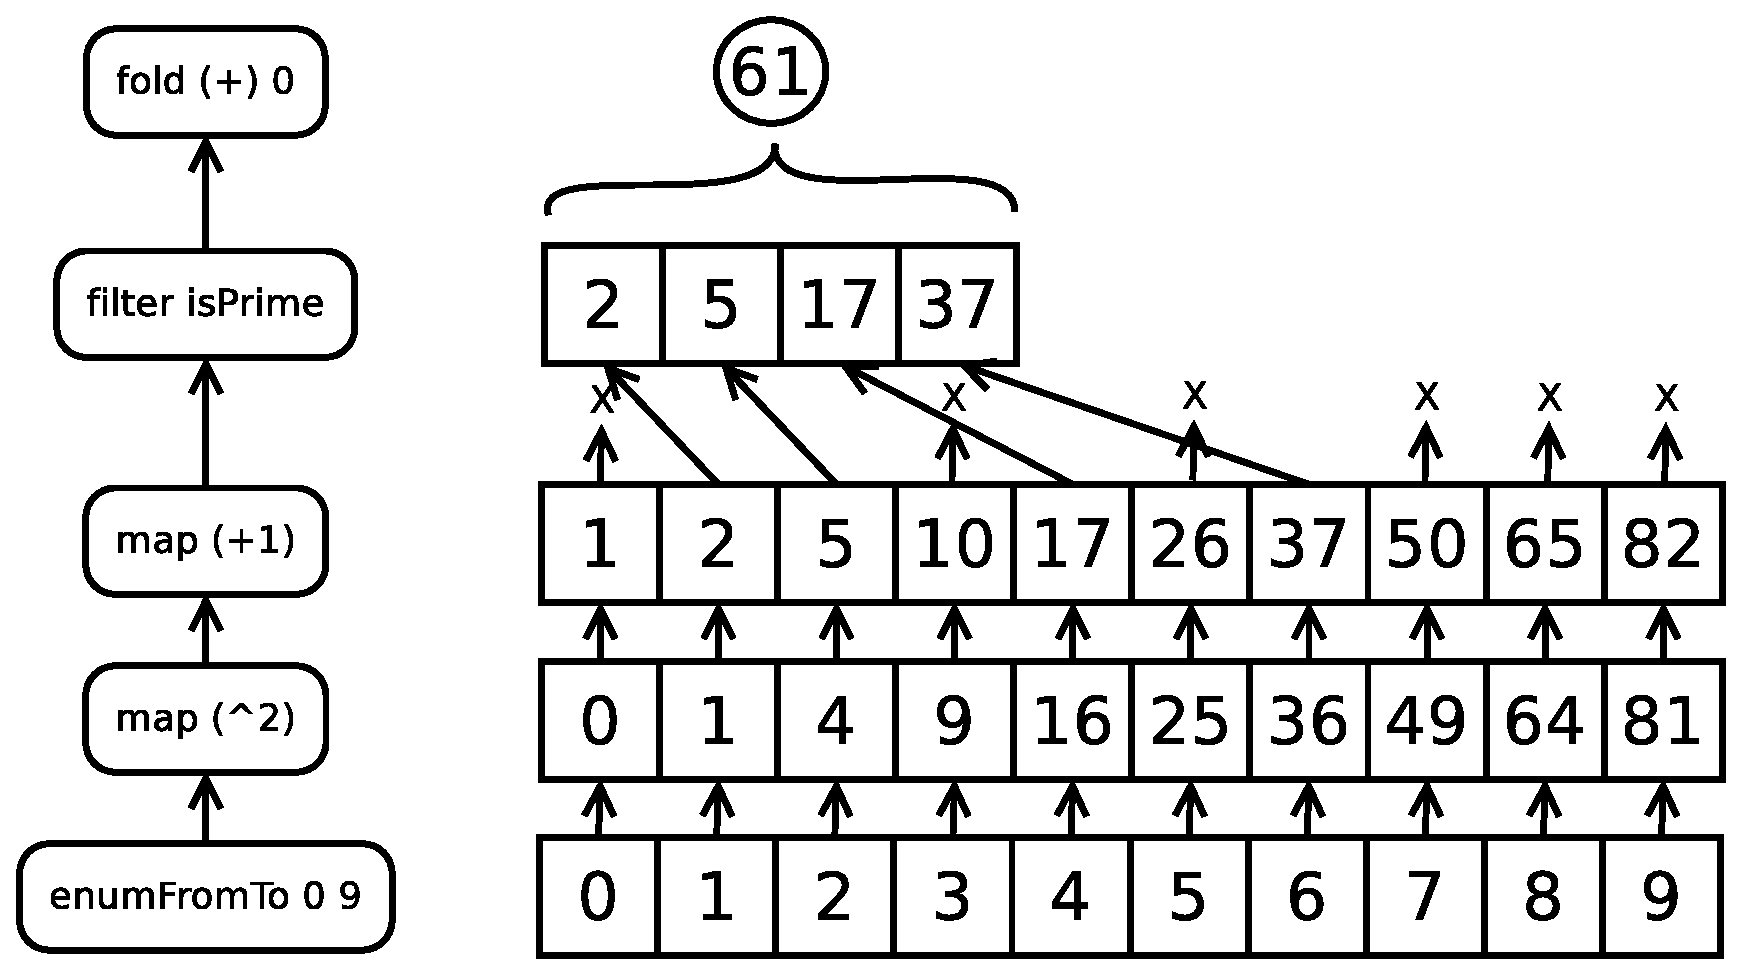
\includegraphics[width=1\textwidth]{img/SumPrimes}

\caption{\label{fig:Prime-Sum-evaluation}{Prime Sum evaluation tree. Delayed evaluation tree (left) and values at every step (right).}}
\end{figure}


In the above example we have an enumeration which always produces and array but consumes none. This functions of this type are called generators by the original authors. A more generic name for them is anamorphisms {[}bananas{]}. These functions are used to bring arrays into the scope of array operations.

The dual of anamorphisms are catamorphisms, or reductions, which consume array(s) and only return scalar values. Folds are one example of such functions.

Most of the functions in the library, however, are hylomorphism which means they consume and produce at least one array. If fusion is not used, each of such functions would allocate a new array and fill it in before the next combinator consumes the newly created array. It is desirable to avoid this. The way Functional Array Fusion looks at this problem is it considers the computation as a pipeline of array combinators, whereby each element is consumed in a lockstep and is directly projected to the correct position in the resulting array. As the right of Figure \vref{fig:Prime-Sum-evaluation} suggests, each element is visualised as being \emph{mutated} in some way to produce the final result. Thus, for each new element @enumFromTo@ generates it is first squared, then incremented by one. It is then run through the predicate of the filter and is taken into account when folding to the final value if found to be true.

The way in which the original authors approached the problem was to generalise generators, reductions and producer/consumers to a small set of combinators covering most of the library interface. They came up with the @loop@ combinator of the following type (adjusted to be consistent with the rest of this document):

\begin{hscode}
loop :: (e -> a -> (Maybe e', a)) -- mutator function
     -> a                         -- accumulator
     -> Array e                   -- input array
     -> (Array e', a)
\end{hscode}


The @loop@ combinator traverses the input array @arr@. The mutator function is made generic so as to be able to act as function supplied to @map@, @filter@ and @fold@ combinators. Thus, @map f@ can be implemented as @loop@ with a unit accumulator and the following mutator function:

\begin{hscode}
map_mf :: (e -> a -> (Maybe e', a))
map_mf x acc = (Just (f x), acc)    -- acc unused
\end{hscode}


Similarly, @filter p@ and @fold f acc@ can be implemented as loops with the following mutator functions:

\begin{hscode}
filt_mf :: (e -> a -> (Maybe e', a))
filt_mf x acc = (filt, acc)         -- acc unused
  where filt = case (p x) of
                 True  = Just x
                 False = Nothing

fold_mf :: (e -> a -> (Maybe e', a))
fold_mf x acc = (Nothing, f x acc)  -- no elt produced
\end{hscode}


It should be noted from the above that the @loop@ combinator is able to express both hylomorphisms (@map@, @filter@) and catamorphisms (@fold@). The latter are identified by the @Nothing@ value unconditionally returned by the \emph{mutator function.} The only function from the original example that is left to be defined in terms of the @loop@ combinator is the anamorphism @enumFromTo@. Its mutator function might\footnote{The library implementation generalises enumerations to \code{enumFromStepLen}, which takes a value for the first element, the increment and desired length of the resulting sequence. } take the following form:

\begin{hscode}
enum_mf :: (e -> a -> (Maybe e', a))
enum_mf _ acc = (Just acc, acc+1)   -- acc is next val
\end{hscode}


The above implementation of @enum@ suggests that it might be possible to express generators using the generic @loop@ combinator. However, a careful reader may have noticed that @loop@, by definition, traverses \emph{an array}, even though the value of the element is ignored in this particular mutator function. Thus, a cheap but generic implementation of generators would have been possible if we had a dummy array to iterate over. As discussed previously in Section \ref{sec:DPH-Data-Representation}\vpageref{sec:DPH-Data-Representation} an array of units can be represented by a single value -- its length. Indexing the array at any position within the bounds would just return a unit value. Now, a generator like @enumFromTo@ could be easily and cheaply implemented as follows:

\begin{hscode}
enumFromTo :: Int -> Int -> Array Int
enumFromTo start end = fst (loop enum_mf start units)
  where units = replicate (end - start + 1) ()
\end{hscode}


In the above implementation an array of units is first constructed by replicating (repeating) a unit value the desired number of times. It is then traversed using the appropriate mutator function resulting in a tuple with the desired enumeration in the first position and the final accumulator in the second (@end+1@ in this case). We can safely drop the accumulator as we are only interested in the array.

The true convenience of the @loop@ combinator is revealed if we try to squash multiple @loop@ combinators into a single @loop@. GHC's rewrite rules mechanism is employed to pipeline two adjacent @loop@s. For the sake of being concise we will omit here most of the infrastructure required for the approach to work. We present the way by which two mutator functions can be merged into a single one:

\begin{hscode}
-- mutator function of the first loop
mf1 :: e0 -> a1 -> (Maybe e1, a1)

-- mutator function of the second loop
mf2 :: e1 -> a2 -> (Maybe e2, a2)
\end{hscode}


\begin{hscode}
-- mutator function to express
-- loop mf2 .. (loop mf1 .. (..)) as a single loop
mf :: e0 -> (a1,a2) -> (Maybe e2, (a1,a2))
mf x (acc1, acc2) =
  case (mf1 x0 acc1) of
    (Nothing, acc1') = (Nothing, (acc1', acc2))
    (Just x1, acc1') =
      case (mf2 x1 acc2) of
        (Nothing, acc2') = (Nothing, (acc1', acc2'))
        (Just x2, acc2') = (Just x2, (acc1', acc2'))
\end{hscode}


Since the mutator function may not always return a value (e.g. in the case with @filter@ combinator) merging two mutator functions proceeds in two steps:
\begin{enumerate}
\item We first run the given array element through the first mutator function. If that does not produce a value (produces a @Nothing@) we do not proceed to the second mutator and yield @Nothing@ as the overall result.
\item In case the first mutator did produce a value (@Just x1@) we run it through the second mutator, returning the final result.
\end{enumerate}
Clearly, some trickery is involved in dropping the first accumulator in a (potentially deeply nested) pair, but the above conveys the main concepts behind the Functional Array Fusion.
\end{comment}

\IfNotCompilingAll{\bibliography{bib}}

\end{document}